\section{Thuật toán Brute Force}

\subsection{Đặc điểm chính}

\begin{itemize}
    \item Không cần pha tiền xử lý.
    \item Bộ nhớ sử dụng là hằng số $O(1)$.
    \item Độ phức tạp thời gian pha tìm kiếm là $O(nm)$ trong trường hợp xấu nhất.
\end{itemize}

\subsection{Mô tả thuật toán}

Thuật toán Brute Force kiểm tra tất cả vị trí trong đoạn văn bản từ vị trí
$0$ đến $n - m$, xem liệu mẫu có khớp tại vị trí đó hay không.
Tại mỗi vị trí $j$, thuật toán so sánh lần lượt từng ký tự của mẫu $x$
với các ký tự tương ứng trong văn bản $y$. Sau mỗi lần kiểm tra,
mẫu được dịch sang phải $1$ vị trí.

Cụ thể, quá trình tìm kiếm diễn ra như sau:

\begin{enumerate}
    \item Bắt đầu từ vị trí đầu tiên của văn bản và trượt cửa sổ mẫu
          qua toàn bộ văn bản.
    \item Tại mỗi vị trí, so sánh lần lượt các ký tự của mẫu với các
          ký tự tương ứng trong văn bản.
    \item Nếu phát hiện sự không khớp, dịch cửa sổ mẫu sang phải một vị trí.
    \item Lặp lại bước 2 và 3 cho đến khi cửa sổ mẫu đạt đến vị trí
          cuối cùng có thể trong văn bản.
    \item Nếu tất cả các ký tự trong mẫu khớp hoàn toàn với các ký tự
          tương ứng trong văn bản, ghi lại vị trí bắt đầu của lần khớp đó.
    \item Dịch cửa sổ mẫu sang phải một vị trí và tiếp tục quá trình
          so sánh.
\end{enumerate}

\subsection{Cài đặt bằng C++}

\begin{verbatim}
#include <iostream>
#include <vector>
using namespace std;

// Hàm tìm kiếm xâu mẫu x trong xâu y
vector<int> bruteForce(string y, string x) {
    vector<int> result;

    int n = y.size();
    int m = x.size();

    // Duyệt từng vị trí có thể
    for (int i = 0; i <= n - m; i++) {
        int j = 0;

        // So sánh từng ký tự
        while (j < m && y[i + j] == x[j]) {
            j++;
        }

        // Nếu khớp toàn bộ pattern
        if (j == m) {
            result.push_back(i);
        }
    }

    return result;
}

int main() {
    string y = "ababcabcabababd";
    string x = "ababd";

    vector<int> pos = bruteForce(y, x);

    cout << "Vi tri xuat hien: ";
    for (int p : pos) {
        cout << p << " ";
    }

    return 0;
}
\end{verbatim}

\subsection{Kiểm nghiệm thuật toán}

Giả sử ta có hai xâu ký tự $y$ (văn bản) và $x$ (mẫu).
Ta tiến hành tìm kiếm xâu $x$ trong xâu $y$ theo từng bước minh họa dưới đây.

\begin{center}
    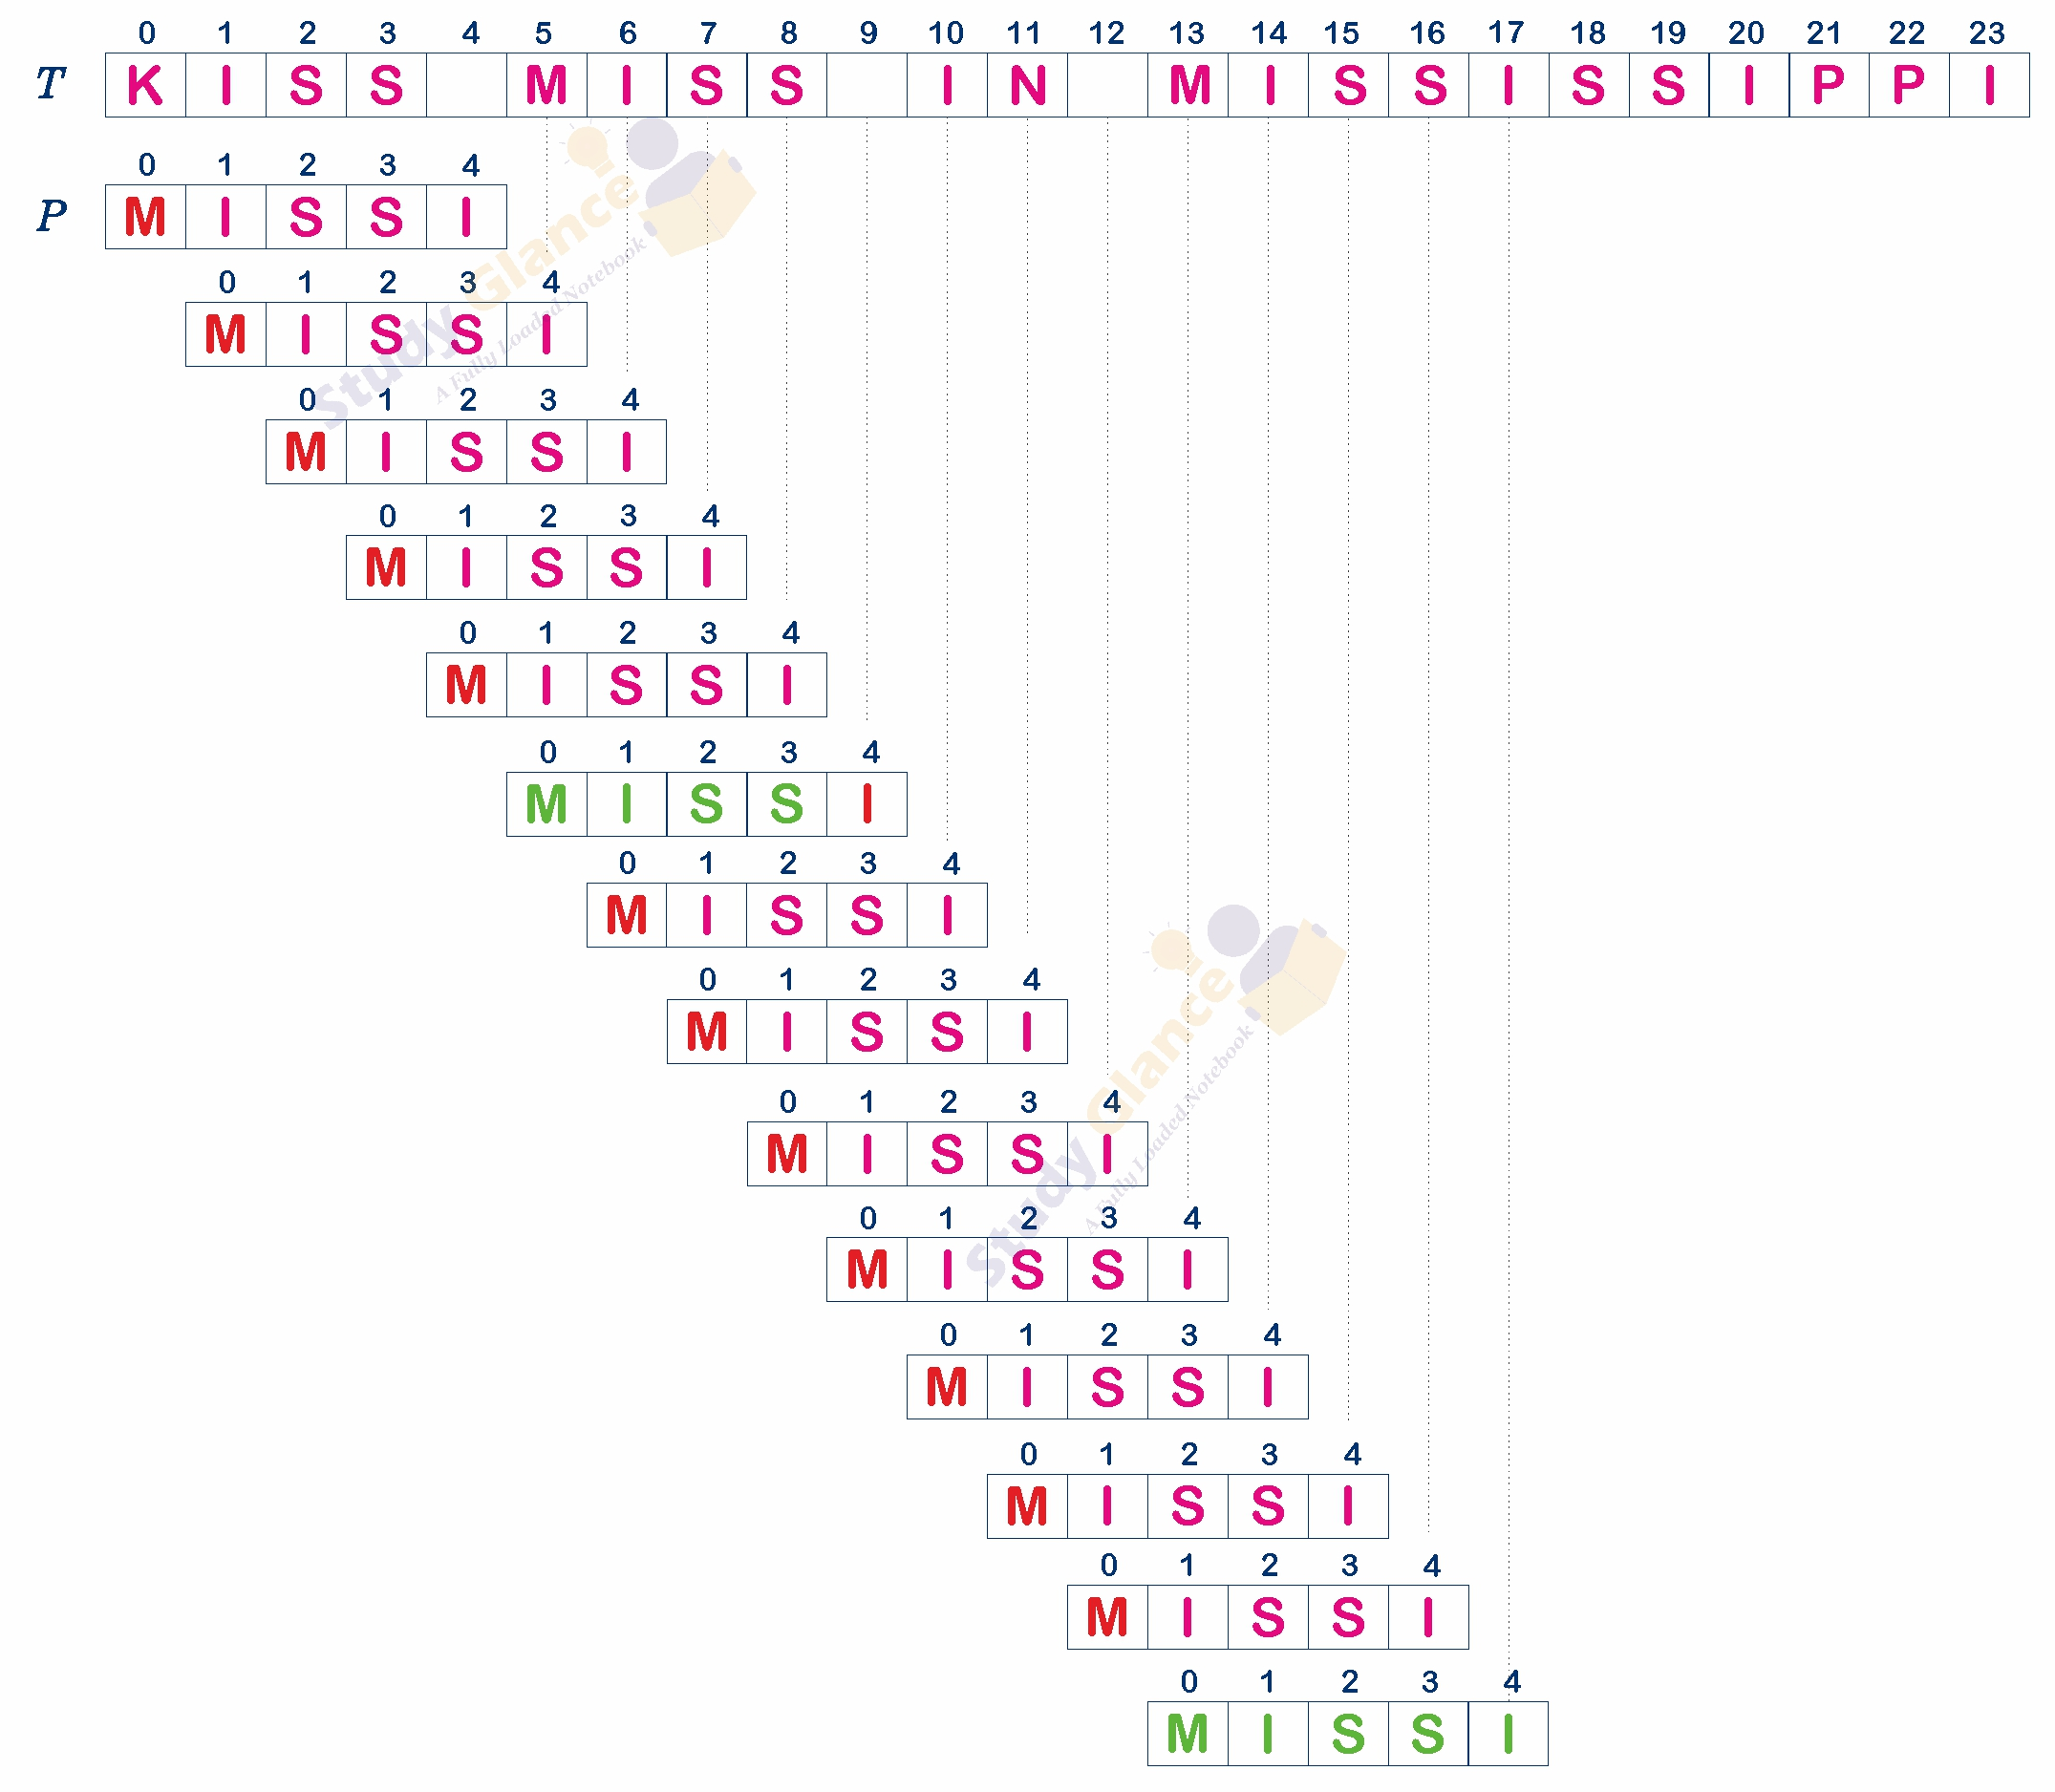
\includegraphics[width=15cm]{Images/Brute-Force-Algorithm.jpg}
\end{center}